\documentclass[a4paper,12pt]{article}

% Paket za slovenski jezik
\usepackage[utf8]{inputenc}
\usepackage[slovene]{babel}

% Matematični paketi
\usepackage{amsmath, amssymb}
\usepackage{geometry}
\geometry{margin=2.5cm}

% TikZ in PGFPlots za risanje grafov
\usepackage{tikz}
\usepackage{pgfplots}
\pgfplotsset{compat=1.18}

\title{Ponovitev kvadratne funkcije}
\author{Vaje za utrjevanje}
\date{\today}

\begin{document}

\maketitle

\section{Naloge}

\subsection*{1. Risanje grafov kvadratnih funkcij}
Določi ničli, teme in začetno vrednost ter nariši graf funkcije:
\begin{enumerate}
    \item $f(x) = x^2 - 4x + 3$
    \item $f(x) = -2x^2 + 4x + 6$
\end{enumerate}

\subsection*{2. Iskanje enačbe iz temena in točke}
Zapiši enačbo kvadratne funkcije v vseh treh oblikah, če sta podana teme $T$ in točka $A$:
\begin{enumerate}
    \item $T(1, -4)$ in točka $A(3, 0)$.
    \item $T(-2, 3)$ in točka $B(0, -1)$.
\end{enumerate}

\subsection*{3. Iskanje enačbe iz ničel in točke}
Zapiši enačbo kvadratne funkcije v vseh treh oblikah, če sta podani ničli $x_1, x_2$ in točka $C$:
\begin{enumerate}
    \item $x_1 = 1, x_2 = 5$ in točka $C(0, 5)$.
    \item $x_1 = -2, x_2 = 4$ in točka $D(1, -9)$.
\end{enumerate}

\newpage

\section{Rešitve}

\subsection*{Rešitve 1. sklopa (Grafi)}

\textbf{1. naloga:} $f(x) = x^2 - 4x + 3$ \\
Ničli: $(x-1)(x-3)=0 \Rightarrow x_1=1, x_2=3$. \\
Teme: $p = \frac{1+3}{2} = 2, q = f(2) = 4-8+3 = -1 \Rightarrow T(2, -1)$. \\
Začetna vrednost: $f(0) = 3$.

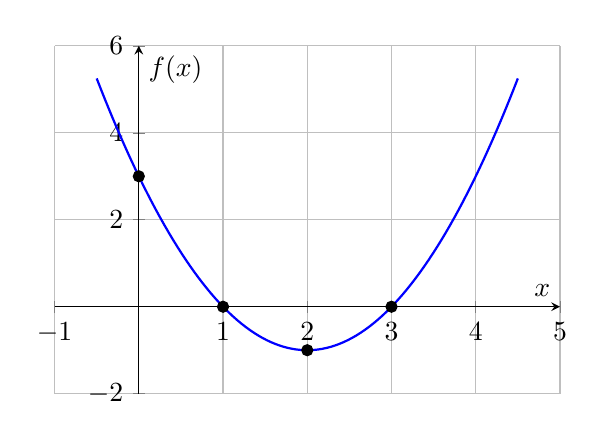
\begin{tikzpicture}
\begin{axis}[
    axis lines = middle,
    xlabel = $x$,
    ylabel = {$f(x)$},
    xmin=-1, xmax=5,
    ymin=-2, ymax=6,
    grid = both,
    width=8cm, height=6cm
]
\addplot [domain=-0.5:4.5, samples=100, color=blue, thick] {x^2 - 4*x + 3};
\addplot[only marks, mark=*] coordinates {(1,0) (3,0) (2,-1) (0,3)};
\end{axis}
\end{tikzpicture}

\textbf{2. naloga:} $f(x) = -2x^2 + 4x + 6$ \\
Ničli: $-2(x^2 - 2x - 3) = -2(x-3)(x+1) = 0 \Rightarrow x_1=3, x_2=-1$. \\
Teme: $p = 1, q = f(1) = 8 \Rightarrow T(1, 8)$. \\
Začetna vrednost: $f(0) = 6$.

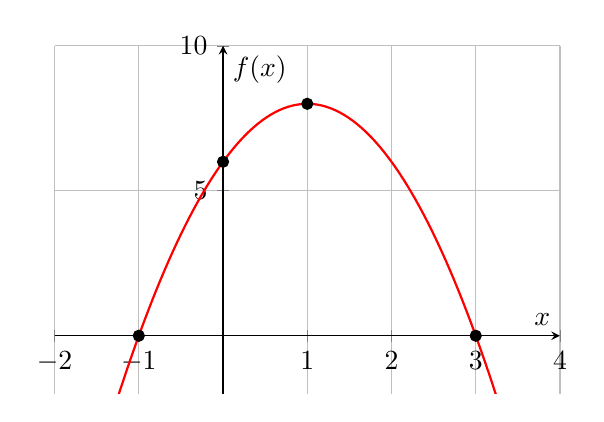
\begin{tikzpicture}
\begin{axis}[
    axis lines = middle,
    xlabel = $x$,
    ylabel = {$f(x)$},
    xmin=-2, xmax=4,
    ymin=-2, ymax=10,
    grid = both,
    width=8cm, height=6cm
]
\addplot [domain=-1.5:3.5, samples=100, color=red, thick] {-2*x^2 + 4*x + 6};
\addplot[only marks, mark=*] coordinates {(-1,0) (3,0) (1,8) (0,6)};
\end{axis}
\end{tikzpicture}

\subsection*{Rešitve 2. sklopa (Teme)}

\begin{enumerate}
    \item $T(1, -4), A(3, 0)$: \\
    Uporabimo temensko obliko: $y = a(x-1)^2 - 4$. \\
    Vstavimo točko $A$: $0 = a(3-1)^2 - 4 \Rightarrow 4 = 4a \Rightarrow a=1$. \\
    Enačba: $f(x) = (x-1)^2 - 4 = x^2 - 2x - 3 = (x-3)(x+1)$.

    \item $T(-2, 3), B(0, -1)$: \\
    $y = a(x+2)^2 + 3$. \\
    Vstavimo $B$: $-1 = a(0+2)^2 + 3 \Rightarrow -4 = 4a \Rightarrow a=-1$. \\
    Enačba: $f(x) = -(x+2)^2 + 3 = -x^2 - 4x - 1$.
\end{enumerate}

\subsection*{Rešitve 3. sklopa (Ničle)}

\begin{enumerate}
    \item $x_1=1, x_2=5, C(0, 5)$: \\
    Uporabimo ničelno obliko: $y = a(x-1)(x-5)$. \\
    Vstavimo $C$: $5 = a(0-1)(0-5) \Rightarrow 5 = 5a \Rightarrow a=1$. \\
    Enačba: $f(x) = (x-1)(x-5) = x^2 - 6x + 5$.

    \item $x_1=-2, x_2=4, D(1, -9)$: \\
    $y = a(x+2)(x-4)$. \\
    Vstavimo $D$: $-9 = a(1+2)(1-4) \Rightarrow -9 = -9a \Rightarrow a=1$. \\
    Enačba: $f(x) = (x+2)(x-4) = x^2 - 2x - 8$.
\end{enumerate}

\end{document}
